\section{RF Front-End Mezzanines}\label{rf-front-end-mezzanines}

Mezzanines providing analogue front-ends (AFEs) for the ADCs and DACs on
Sayma.

\section{Available AFEs}\label{available-afes}

\subsection{TestMod}\label{testmod}

Simple mezzanine designed for thermal and connectivity testing, and to
serve as a template for other mezzanine designs.

\todo[inline]{image}

Design files are
\href{https://github.com/m-labs/sinara/tree/master/ARTIQ_ALTIUM/Sayma_AFEs/TestMod}{here},
the schematic is
\href{https://github.com/m-labs/sinara/tree/master/ARTIQ_ALTIUM/Sayma_AFEs/TestMod/AFE_mezzanine.PDF}{here}.


\subsection{BaseMod}\label{basemod}

BaseMod is a base-band input/output mezzanine. Design files are
\href{https://github.com/m-labs/sinara/tree/master/ARTIQ_ALTIUM/Sayma_AFEs/BaseMod}{here}.
\todo[inline]{there are no sch in pdf}
%the schematic is
%\href{https://github.com/m-labs/sinara/blob/master/ARTIQ_ALTIUM/PCB_mezzanine_analog_allaki/Project\%20Outputs\%20for\%20allaki_mezzanine/allaki_mezzanine.PDF}{here}.

NB: 12/2017 Allaki was
\href{https://github.com/m-labs/sinara/issues/396}{renamed} BaseMod.

\todo[inline]{image}

\subsubsection{Outputs}\label{outputs}

BaseMod provides two independent RF outputs, featuring:

\begin{itemize}

	\item
	\textbf{Bandwidth}: 10MHz - 4GHz (upper frequency is limited by
	several different components)
	\item
%	\textbf{Max output power}: ?dBm (limited by ?).
	\item
	\textbf{Output filters}: either 3 Mini-Circuits FV1206 series filters,
	or a user-definable discrete 9-pole discrete-element filter using 0402
	components.
	\item
	\textbf{Low phase noise amplifier}: Mini-Circuits ERA-4XSM+); 14.2dBm
	gain at 1GHz.
	\item
	\textbf{Digitally programmable attenuator}: HMC542BLP4E; 0dB to 31.dB
	in 0.5dB steps; controllable in real-time.
	\item
	\textbf{Fast, high-isolation RF switch}: HMC349LP4C; 67dB isolation at
	1GHz; controllable in with real-time control.
	\item
	\textbf{Power detector}: AD8363ACPZ on switch ``off'' port for
	monitoring and power levelling.
	\item
	\textbf{Optional isolation of output grounds}: to avoid ground loops,
	achieved by fitting capacitors and washers.
\end{itemize}

\subsubsection{Inputs}\label{inputs}

BaseMod provides two independent inputs, each of which can be configured
(component placement) as:

\begin{enumerate}
	\def\labelenumi{\arabic{enumi}.}
	\item
	Direct feed to ADC via ADA4927-1 buffer for maximum bandwidth
	\item
	Low-noise programmable gain instrumentation amplifier (AD8253)
	front-end
\end{enumerate}

\begin{itemize}
	\item
	\textbf{Bandwidth}: DC-300kHz
	\item
	\textbf{Input ranges}: ±0.1V, ±1V, ±10V
	\item
	\textbf{Fully differential inputs}: 100k between each input signal and
	ground and the circuit ground
	\item
	\textbf{Filters}: Common-mode and differential mode filtering of RF
	interference for optimum DC precision
	\item
	\textbf{Input protection}: diodes between each input and the supply
	rails for maximum ruggedness
	\item
	Supports both high-speed input directly coupled into a high-speed
	pre-amp, and low-frequency inputs using a variable-gain
	instrumentation amplifier (choice by component selection). Pull
	details from \href{https://github.com/m-labs/sinara/issues/81}{\#81}
	\item
	Instrumentation amp: gain, filters, etc.
\end{itemize}

\subsection{MixMod}\label{mixmod}

MixMod is an up-converting mezzanine, using an analogue IQ mixer to mix
the input and output RF signals with a LO supplied by Sayma.

The LO provided by Sayma should be a 3V3 PECL square-wave.

Design files are
\href{https://github.com/m-labs/sinara/tree/master/ARTIQ_ALTIUM/Sayma_AFEs/MixMod}{here}
\href{https://github.com/m-labs/sinara/tree/master/ARTIQ_ALTIUM/Sayma_AFEs/BaseMod}{here}.
\todo[inline]{there are no sch in pdf}
\todo[inline]{image}

\subsubsection{Outputs}\label{outputs-1}

MixMod provides a single RF output between 2.5GHz and 3.5GHz, produced
by mixing two DAC channels with a LO supplied by Sayma. Other than the
IQ mixer, the output signal-chain is identical to BaseMod.

\subsubsection{Inputs}\label{inputs-1}

MixMod's two inputs can either be operated in baseband or downconversion
mode (selectable by component choice). In baseband mode, the inputs
function identically to BaseMod's. In downconversion mode, a single SMA
input feeds the RF port on an IQ mixer to produce a pair of baseband
signals, which then feed the two signal chains.

\section{Mezzanines Mechanical Specification}\label{general-specification}


\begin{itemize}

	\item Board size
		\begin{figure}[htbp!]
			\centering
			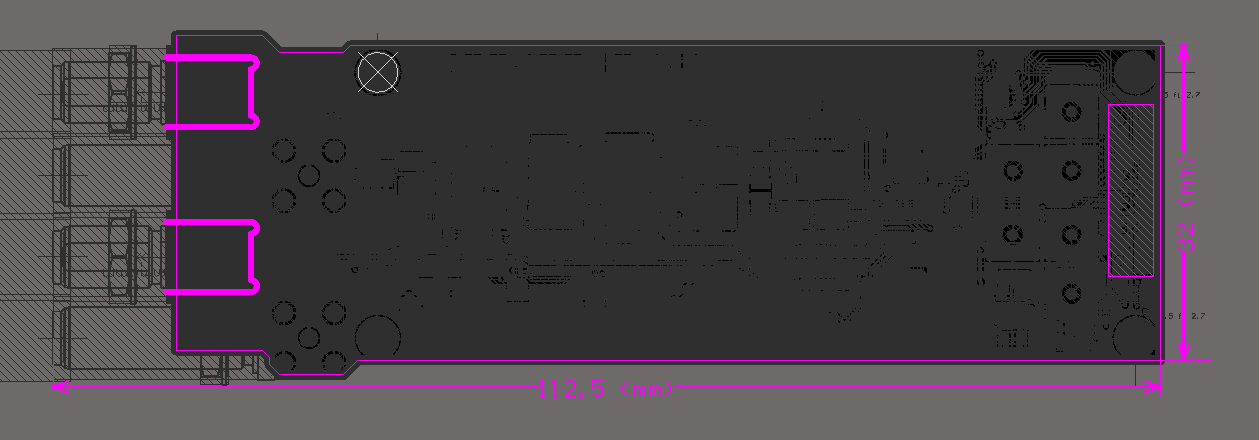
\includegraphics[width=17cm]{img/MEZZ.png}\\
			\caption{Mezzaninne dimensions}
		\end{figure}	
	\item Mounting holes\\
	There are four mounting holes fi 2.7mm for M2.5 screws.
%	\item
%	SMA locations and pns
%	\item
%	Connectors
\end{itemize}

%\subsection{Electrical}\label{electrical}
%
%\begin{itemize}
%
%	\item
%	Suggest
%	\href{http://www.analog.com/en/products/rf-microwave/iq-modulators-demodulators/iq-modulators/adl5375.html}{ADL5375}
%	IQ modulator. Good intrinsic carrier/sideband rejection, relatively
%	low temp coefficients, sufficient IF bandwidth, good I/Q linearity.
%	This is the chip used in the NIST Magtrap drive system.
%\end{itemize}
